\begin{otherlanguage}{french}
\subsubsection*{\centering{Résumé long}}
\subsection*{FastTrack un logiciel de tracking généraliste}
\subsubsection*{Introduction}
Le tracking d'objets depuis des enregistrements vidéos est un problème qui a gagné en popularité, tant dans l'industrie quand dans le milieu académique. Citons par exemple le projet ATTOL d'Airbus qui permet le roulage, le décollage et l'atterrissages d'un avion en se basant uniquement sur de l'analyse d'image. Dans le milieu académique, le tracking sur vidéos est très utilisé en biologie et en écologie. Il permet de suivre les animaux dans leur environnement sans avoir besoin de les marquer invasivement.

En se concentrera dans cette thèse sur le tracking d'objets multiples (MOT) qui regroupe la majorité des applications scientifiques. Le tracking d'objets multiples est un problème qui consiste à détecter et à garder l'identité des objets tout au long d'un enregistrement vidéo. C'est un problème complexe sous plusieurs aspects: la détection des objets peut être compliquée si par exemple ceux si disparaissent derrière des objets du décor, de plus la qualité des images influence grandement la détection. Les objets peuvent sortir et rentrer dans le champ de vue où se superposer ce qui complique le maintient de l'identité de chaque objet.

On distingue deux grandes classes d'algorithmes permettant de solutionner ces problèmes. Le premier utilise les paramètres cinématiques de l'objet ce qui permet ainsi de prédire et retrouver l'identité des objets d'une image sur l'autre. Très rapide, cette classe d'algorithmes souffre d'un problème majeur, la propagation des erreurs. Si une erreur est commise sur une image, elle se propagera jusqu'à la fin du film. La deuxième classe d'algorithmes utilise une "carte d'identité" extraite pour chaque objet. Cela permet de contourner le problème de propagation des erreurs au prix d'un temps de calcul très élevé.

Plusieurs logiciels de tracking existent. On peut citer Ethovision XT, Any-maze et ToxTrack pour les logiciels propriétaires. Les deux premiers sont livrés clef-en-mains mais coûtent cher ce qui peut être un frein pour certains laboratoires. Ces logiciels sont closed-source, c’est-à-dire qu'on ne peut ni les modifier, ni savoir exactement comment ils fonctionnent, ils ne pourront donc pas être adaptés pour un projet particulier. Dans les logiciels open-sources, on peut citer DeepLabCut, idTrackerai et idtracker. Les deux premiers utilisent le machine learning pour effectuer le tracking. Dans les trois cas, ces logiciels nécessitent des ordinateurs puissants et le tracking est en général long, l'installation est en général complexe et nécessite de bonnes connaissances en informatique.

\subsubsection*{Dataset}
Nous avons en premier lieu regroupé divers films pouvant servir de test pour les algorithmes de tracking. Ce dataset nommé The Two Dimentionnal Dataset $TD^2$ regroupent 41 films de plus de 7 espèces animales allant du poisson à la drosophile, des particules actives, des gouttes microfluidique et des objets macroscopiques comme des voitures et des joueurs d'ultimate.

\subsubsection*{FastTrack}
Pour répondre au problème du tracking d'objets multiples, nous avons développé un logiciel nommé FastTrack. Ce logiciel est basé sur une approche inédite du tracking : au lieu de développé un système très spécifique qui ne sera utilisable que sur un très petit nombre de systèmes, FastTrack implémente un algorithme de tracking généraliste utilisable sur une grande variété de systèmes, un outil ergonomique de gestions des erreurs est ensuite proposé pour que l'utilisateur puissent corriger le tracking.

Le workflow de FastTrack peut être divisé en 3 étapes. La première consiste à détecter les objets. Ceci est fait en calculant et soustrayant le fond aux images puis en appliquant un seuil. FastTrack intègre les opérations d'analyses d'image usuelle pour faciliter la détection. Les objets sont ensuite triés par taille ce qui permet d'écarter les artéfacts. Dans une deuxième étape, les objets sont assignés d'une image sur l'autre ce qui permet de garder leurs identités. Ceci est fait en calculant une fonction de coût et en la minimisant pour trouver l'assignation optimale. La fonction de coût comprend le déplacement, le changement d'orientation, de taille et de périmètre des objets entre deux images successives et peut être réglé par l'utilisateur au moyen d'un ensemble de paramètres de normalisation. Deux autres paramètres de seuil permettre de définir une mémoire et une taille maximale d'assignation. La troisième et dernière étape est la correction manuelle des erreurs qui se fait dans un environnement interactif et ergonomique.

    \begin{figure}[h!]
      \centering
      \includegraphics[width=1\textwidth]{part_1/assets/Figure_1_fr.png}
        \caption{{\bf FastTrack flux de traitement} Le flux de traitement se divise en 3 étapes: la détection, l'association, et la correction. Les \faUser indiquent les étapes nécessitant l'utilisateur (film: $ZFJ\_001$.)}
      \label{}
    \end{figure}

FastTrack permet grâce à cette technique d'être applicable sur un grand nombre de systèmes. Les paramètres de normalisation permettent de l'adapter à n'importe quelle dynamique d'objets. Un jeu de paramètres neutres peut être automatiquement trouvé par le logiciel pour aider l'utilisateur à obtenir un tracking le plus optimal possible. Contrairement aux logiciels existant, FastTrack peut tracker des films à nombre d'objets variable, c’est-à-dire dont les objets peuvent disparaitre puis réapparaitre ou de nouveaux objets rentrer dans le champ de vision. Nous avons montré que les performances de FastTrack sont aussi bonnes que les logiciels existants. De plus, notre approche permet à l'utilisateur de gagner du temps sur la plupart des projets, le temps de correction manuel étant en général plus faible que celui de faire un tracking directement sans erreur avec un algorithme plus couteux en temps de calculs.

Nous avons montré comment nous pouvions classer le dataset en utilisant la probabilité d'incursion. Une incursion survenant lorsque l'objet à tracker sort de sa cellule de Voronoï. La probabilité d'incursion peut être défini en utilisant uniquement les propriétés géométriques de l'objet et la distribution des déplacements. Les films peuvent alors être classé suivant leur difficulté de tracking grâce à cette probabilité et ainsi estimer le nombre de corrections manuelles qu'il faudra effectuer. Nous définissons, grâce à cette probabilité un critère permettant de calculer la fréquence d'acquisition optimale qui est une question fréquente lors de la conception d'expériences.

La conception de FastTrack repose sur des bibliothèques et langages ouverts ce qui permet à n'importe qui de voir le code source et de la modifier. FastTrack est entièrement documenté et peut être intégré dans un projet déjà existant. FastTrack dispose d'un système d'intégration et de déploiement continu (CI/CD) grâce au système GitHub Actions. Il est disponible pour Linux (AppImage), MacOs et Windows et facilement installable. Un manuel d'utilisation et des tutoriels vidéos sont disponibles.


\subsection*{Caractérisation de la perception chimique chez le jeune poisson-zèbre}

\subsubsection*{Introduction}
La perception chimique est l'une des plus anciennes modalités sensorielles. Présente dans une grande variété de taxons, des unicellulaires jusqu'aux mammifères, elle est nécessaire à des comportements nécessaire à la survie de l'espèce tels que trouver de la nourriture, se reproduire ou éviter des prédateurs. Les poissons sont baignés dans leur environnement chimique à chaque instant et sont pourvus d'organes pour percevoir et interpréter ces stimulus chimiques. Pour les poissons, la perception chimique passe par l'odorat, le goût et un sens chimique commun. Les mécanismes de perceptions ont été largement étudiés chez diverses espèces de poissons, mais peu est connu sur certains comportements complexes tel que par exemple les migrations.

Le poisson-zèbre est un modèle en plein expansion dans le cadre des neurosciences. La larve est transparente ce qui permet d'observer l'intégralité du cerveau à l'échelle cellulaire grâce à l'image calcique à nappe de lumière. L'apparition de système de réalité virtuelle pour observer le cerveau de larves effectuant des tâches a permis d'élucider des comportements tels que la phototaxie, la capture de proies et la rhéotaxie. L'application de cette technique à la perception chimique nécessite quelques étapes préalables, par exemple une bonne caractérisation des produits et de la réponse comportementale qu'ils entraînent en fonction de la concentration. Pour cela, il est nécessaire d'avoir un dispositif expérimental permettant de faire varier les produits, leurs concentrations ainsi que l'âge du poisson tout en caractérisant leurs préférences. Dans un deuxième temps, un montage permettant de reproduire des écoulements sera nécessaire pour étudier la navigation par perception chimique.

\subsubsection*{Montages expérimentaux}
Pour caractériser la perception chimique chez le jeune poisson-zèbre, nous avons construit deux montages expérimentaux, l'un permettant de faire un criblage des préférences des poissons à divers stimulus chimiques, l'autre permettant de recréer des écoulements réalistes pour étudier la réponse comportementale du poisson.

\paragraph{Dual} Dual est un montage expérimental permettant de quantifier la préférence des poissons vis-à-vis d'un produit chimique de concentration parfaitement contrôlé. Il permet de séparer un compartiment où est placé le poisson en deux zones distinctes, l'un avec un produit de concentration parfaitement connue, l'autre avec de l'eau. Ceci est réalisé grâce à un flux créé par un double pousse-seringue permettant de maintenir un écoulement à volume constant dans le compartiment : quand deux seringues injectent d'un côté, deux seringues aspirent de l'autre. Un système de valves permet de remplir les seringues avec le produit choisi puis d'injecter ensuite. L'aquarium est coupé de l'environnement par une boîte et l'expérience filmée en lumière infrarouge pour éviter toutes implications d'une autre modalité sensorielle, principalement la vision. L'écoulement est visualisé par un colorant infrarouge. Ce montage expérimental est open-source, flexible, et peut être reproduit pour moins de 2 000 euros avec peu de matériel (imprimante 3D et découpe laser). Un logiciel de contrôle open-source est disponible et permet de contrôler le dispositif.

    \begin{figure}[h!]
      \centering
      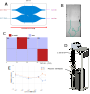
\includegraphics[width=1\textwidth]{part_2/assets/resume1.png}
      \caption{\textbf{A} Schéma du compartiment où nage le poisson. \textbf{B} Image d'un écoulement typique avec en bas le produit visible à l'aide. \textbf{C} Schéma du protocol expérimental permettant de déterminer la préférence des poissons. \textbf{D} Le disposition expérimental Dual. \textbf{D} Préférence index (temps passé dans le produit moins temps passé dans l'eau divisé par le temps total) pour l'ATP en fonction de la concentrentation. On remarque une répulsion au premier cycle P1 (préférence index négatif) et une attraction au cycle P2 (préférence index positif).}
      \label{}
    \end{figure}

\paragraph{The Tropical River} The Tropical River est un montage expérimental qui permet de recréer des écoulements plus réalistes auxquels sont soumis les poissons dans leur environnement naturel. Il est constitué d'un canal de 60×10×10 cm dans lequel est placé le poisson. Un écoulement laminaire contrôlé en température et en débit alimente ce canal. Un système de valves et d'injecteurs permet de créer des jets laminaires et turbulents de manière à étudier la perception chimique du poisson dans un environnement plus proche de la réalité où la perception est fragmentée.

\subsubsection*{Résultats}
Nous avons étudié la préférence de poisson-zèbre âgés de 14 jours et de 7 jours en utilisant Dual. L'expérience dure une heure durant laquelle le poisson est soumis à un cycle avec de l'eau des deux côtés (B1) servant de contrôle, un cycle avec un produit d'un côté et de l'eau de l'autre (P1), un cycle de rinçage similaire à B1, enfin le même cycle que P1 mais en inversant les côtés (P2).

Nous nous sommes concentré sur 5 produits : l'acide citrique et la quinine connues pour être répulsive, l'ATP et l'adénosine connue pour être attractive chez les poissons-zèbres adultes.

En premier lieu nous avons contrôlé que l'expérience ne contenait aucun biais et que le colorant servant à visualiser l'écoulement était bien neutre pour le poisson. Nous avons ensuite montré que les poissons-zèbres étaient repoussés par l'acide citrique, l'intensité variant en fonction de la concentration.

Nous avons trouvé un effet de répulsion à la première présentation d'ATP, puis d'attraction à la seconde présentation chez la majorité des poissons-zèbres âgés de 14 jours. Cette étude effectuée aussi chez les larves de 7 jours manque de statistique mais cet effet ne semble pas être présent. Cela indiquerait une évolution temporelle de ce phénomène absent chez les larves (7 jours), présent chez les adultes (2 mois) et une partie des juvéniles (2 semaines).
\end{otherlanguage}
